\FloatBarrier
\section{Image Processing}
\label{sec::33_ip}
In the previous sections, we have learned about two different approaches to train neural nets on solving certain tasks. Although we came to understand that the complexity of the task to be solved correlates strongly with the amount of data at hand, there exist domains from which it is undeniably easier to do so. To equip a neural network with some prior knowledge by switching the domain may therefore not only be highly desirable but sometimes also needed if the amount or quality of data is not sufficient. One domain which is of special interest when it comes to interacting in a three-dimensional environment is a domain that represents depth information. If there are any, it may sometimes be possible to extract this kind of prior knowledge from a depth camera. As for this work, we need to rely on stereo cameras and powerful algorithms that allow us to compute depth images in real-time. The algorithm that helps us to do so, in terms of the extraction of weighted least squares disparity maps \cite{min2014fast}, will be presented in the following paragraph - Depth Map Extraction.
\FloatBarrier
\subsection{Depth Map Extraction}
As already pointed out, the depth map is generated from stereo camera images by a technique called stereo block matching \cite{hamzah2010sum}. This method works best for edge filtered images, as will become clear soon. To obtain edge filtered images $\bm{E}$, the stereo RGB images are first converted into grayscale $\bm{G}$, which are then convolved with the Sobel kernel $\bm{S}_x$ along the horizontal axis \cite{sobel2014an} (equation \ref{eq::331_sobel_conv}, figure \ref{fig::331_image_preprocessing}). 
\begin{align}
	\bm{E} = \bm{S}_x*\bm{G}
	\label{eq::331_sobel_conv}
\end{align}
\begin{figure}[h!]
	\centering
	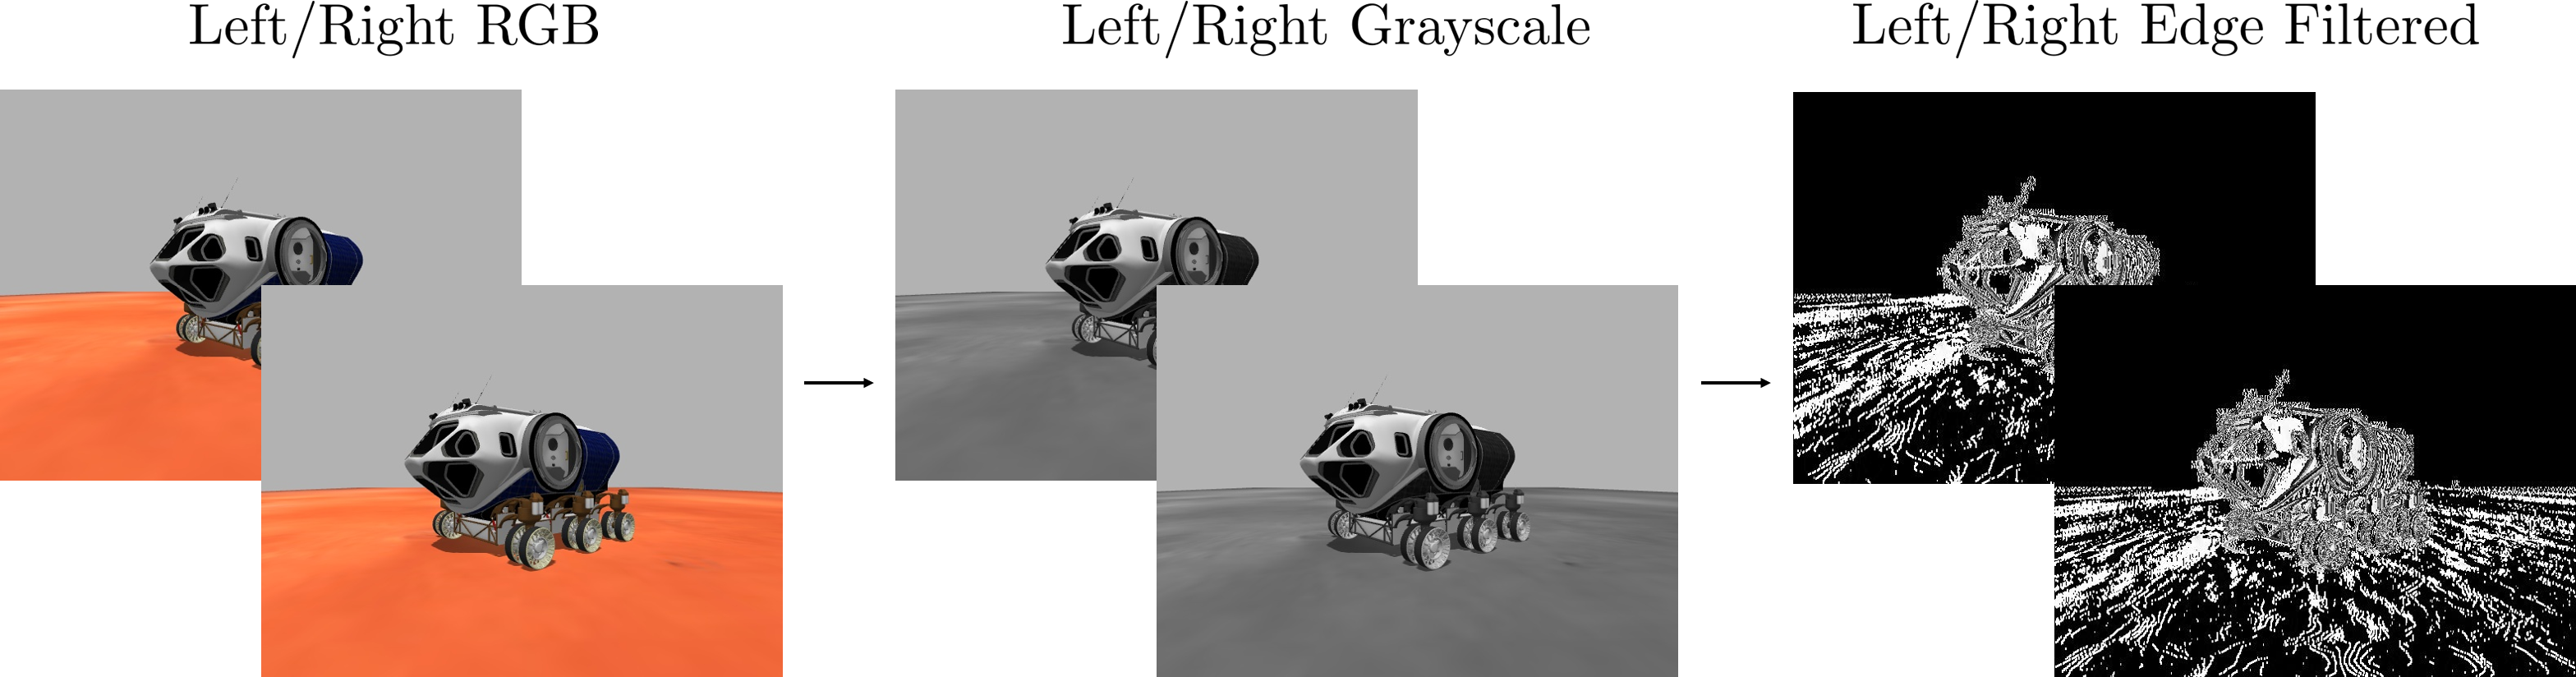
\includegraphics[scale=.28]{chapters/03_fundamentals_of_image_processing/img/image_preprocessing.png}
	\caption{Image pre-processing to obtain edge filtered images. The images were taken within the simulation environment Gazebo (\href{http://gazebosim.org/}{\underline{link}}), and show a space exploration vehicle, for which, with the friendly support of NASA, we generated a Gazebo version (\href{https://github.com/mhubii/gazebo_models}{\underline{link}}).}
	\label{fig::331_image_preprocessing}
\end{figure}
When having a look at the Sobel kernel $\bm{S}_x$ (equation \ref{eq::331_sobel}), it immediately becomes clear that it approximates the derivative of an image along the horizontal axis. Therefore, at locations of steep change, or simply put, edges, the convolution of the grayscale images with the Sobel kernel results in high values, and thus in the typical appearance of an edge filtered image.
\begin{align}
	\bm{S}_x=
	\begin{pmatrix}
		-1 & 0 & +1 \\
		-2 & 0 & +2 \\
		-1 & 0 & +1
	\end{pmatrix}
	\label{eq::331_sobel}
\end{align}
To understand the block matching algorithm, we first need to figure out the transformation that images undergo for a change in perspective, which is caused by the two different positions of the cameras within the stereo camera pair. For an ideal setup, we have two identical cameras, and they are neither rotated relatively to each other, nor is there any other translation, but a shift along the x-axis (figure. \ref{fig::331_stereo_camera}). This may of course not always be true, and there are methods to correct for uncertainties, which we will present in the following paragraph, but omit for simplicity right now. The principle goal, for the inference of depth information from two images, is to find points in the right image that correspond to points in the left image. By triangulation, the displacement or disparity of a point in the right image, relative to its corresponding point in the left image, can then be used to extract the depth. The farther a point $\bm{X}$ lies away from the cameras, the smaller its displacement will be. In figure \ref{fig::331_stereo_camera}, we can see that a point $\bm{X}$, which is seen by the left camera, could in principle lie anywhere on the epipolar line at $\bm{x}'$, as seen from the right camera, if there is no depth information available. 
\begin{figure}[h!]
	\centering
	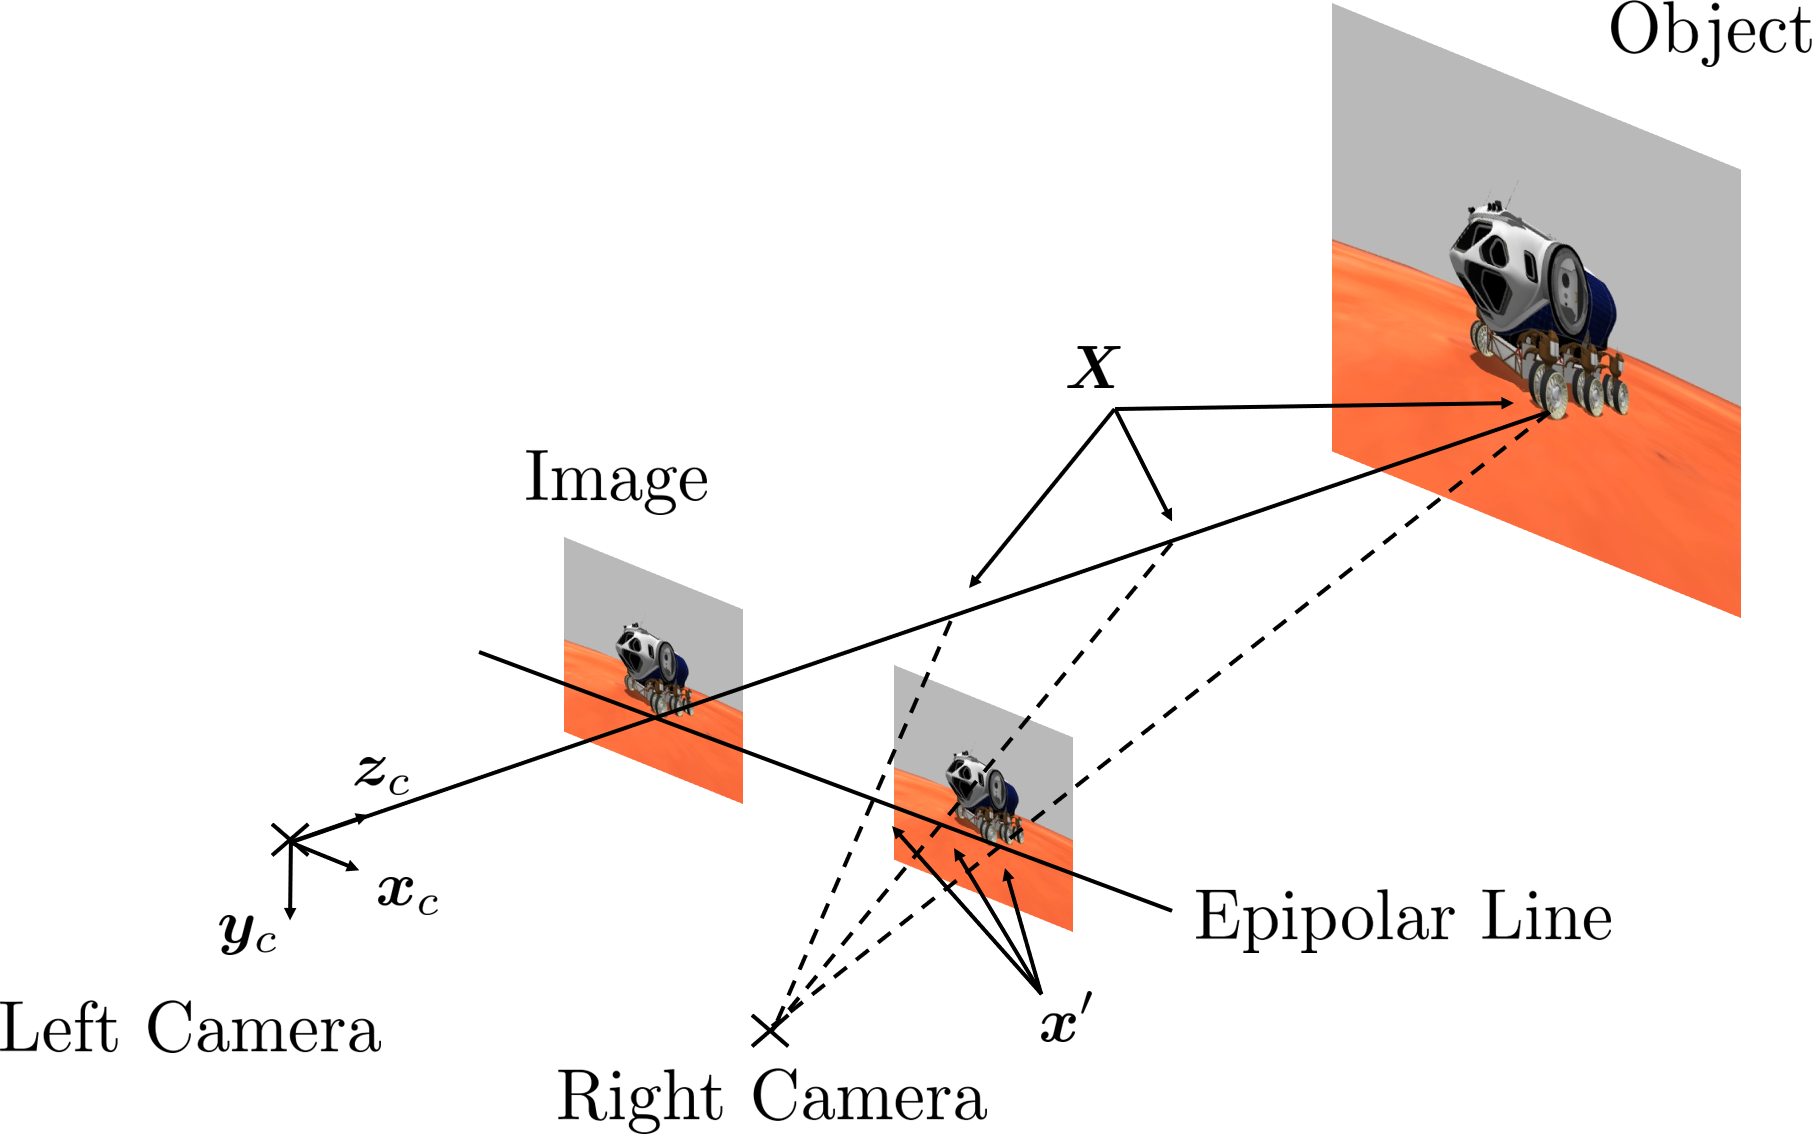
\includegraphics[scale=.28]{chapters/03_fundamentals_of_image_processing/img/stereo_camera.png}
	\caption{The stereo setup with a left and a right camera.}
	\label{fig::331_stereo_camera}
\end{figure}
It results that, to find correspondences, one only must search along the epipolar line. Also, since points in the right image that correspond to points in the left image, will always be displaced to the left, one only must search in this direction. The procedure is shown in figure \ref{fig::331_left_disparity_map}. Instead of looking for single-pixel correspondences, it is advised to search for whole block correspondences, since it reduces the noise drastically. Blocks of a defined block size $N$ are taken from the left image, and then the sum of absolute differences SAD is computed for every displacement $d$ in the right image, ranging from zero to number of disparities $D$ (equation \ref{eq::331_sad}, figure \ref{fig::331_left_disparity_map}).
\begin{align}
	\text{SAD}(d) = \sum_{x,y=0}^N |\bm{E}_\text{left}(x,y) - \bm{E}_\text{right}(x-d,y)|
	\label{eq::331_sad}
\end{align}
The disparity $d$ that minimizes the sum of absolute differences SAD is taken to serve as the best correspondence and is therefore used in the disparity map.  Here we can already see that due to the uniqueness of the edge filtered the images $\bm{E}$, it is easier to find correspondences there, rather than in the grayscale or RGB images.
\begin{figure}[h!]
	\centering
	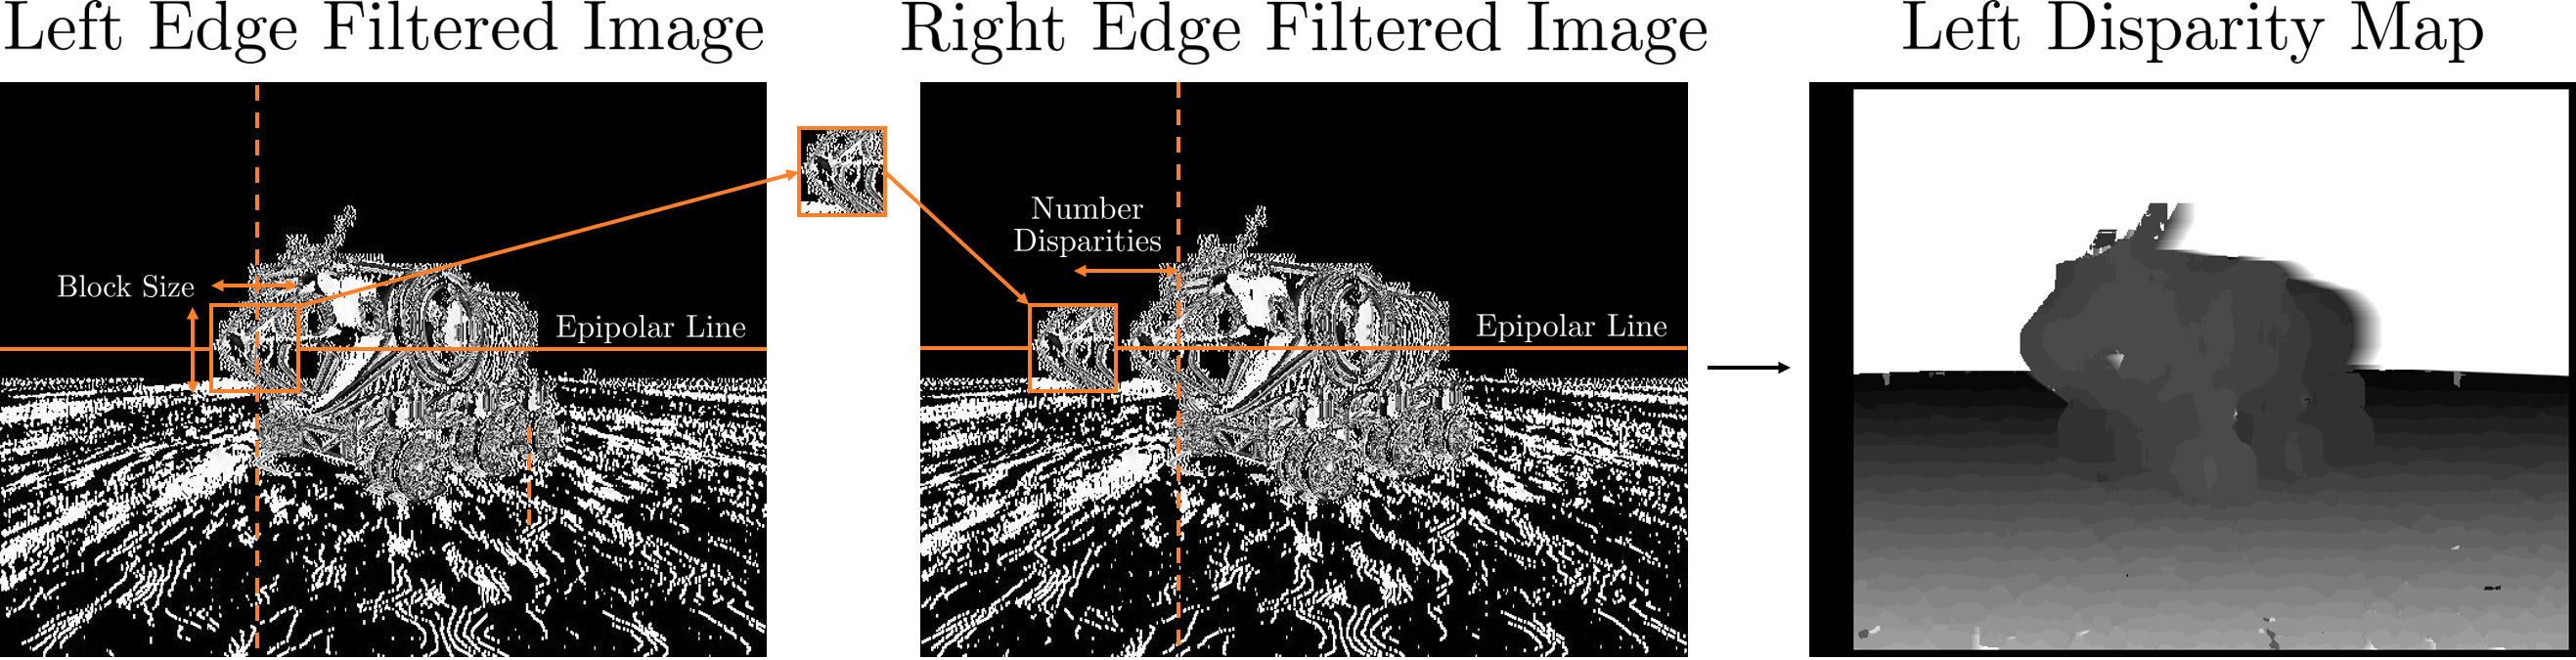
\includegraphics[scale=.28]{chapters/03_fundamentals_of_image_processing/img/left_disparity_map.png}
	\caption{Generation of the left disparity map by the block matching algorithm.}
	\label{fig::331_left_disparity_map}
\end{figure}
To further refine the disparity map, and especially to assure good results in textureless  regions, we apply a weighted least squares filtering, which is based on the confidence of depth measures. The confidence of depth measures is obtained from the variance within the disparity map $\bm{D}$ (equation \ref{eq::331_variance}, figure \ref{fig::331_confidence_map}).
\begin{align}
	 \text{Var}(\bm{D}) = \mathbb{E}\left[\bm{D}^2\right] - \mathbb{E}\left[\bm{D}\right]^2
	\label{eq::331_variance}
\end{align} 
Therein, the expectation value for $\bm{D}$ is computed by a convolution with the kernel $\bm{K}$ from the following equation
\begin{align}
	\bm{K} &= \alpha
	\begin{pmatrix}
	1 & \dots & 1 \\
	\vdots & \ddots & \vdots \\
	1 & \dots & 1
	\end{pmatrix} \\
	\mathbb{E}\left[\bm{D}\right] &= \bm{K}*\bm{D},
	\label{eq::331_kernel}
\end{align}
where $\alpha = \frac{1}{\text{width}\cdot\text{height}}$ is the normalization factor. The expectation value of the disparity map squared $\mathbb{E}\left[\bm{D}^2\right]$ is computed in the same way, except for that all elements are squared prior to summing them up. Given the variance, we can introduce a concept which is named confidence map. The confidence map $\text{Con}(\bm{D})$ is a measure for the certainty of the computed disparity, and is defined to be linearly dependent on the variance as follows
\begin{align}
	\text{Con}(\bm{D}) = \max\left(1-r\text{Var}(\bm{D}),0\right),
\end{align}
where $r$ is a roll-off factor that defines the change of confidence with growing variance. The resulting disparity confidence is shown in figure \ref{fig::331_confidence_map} and is used to outweigh outlying disparity values from the final weighted least squares disparity map. 
\begin{figure}[h!]
	\centering
	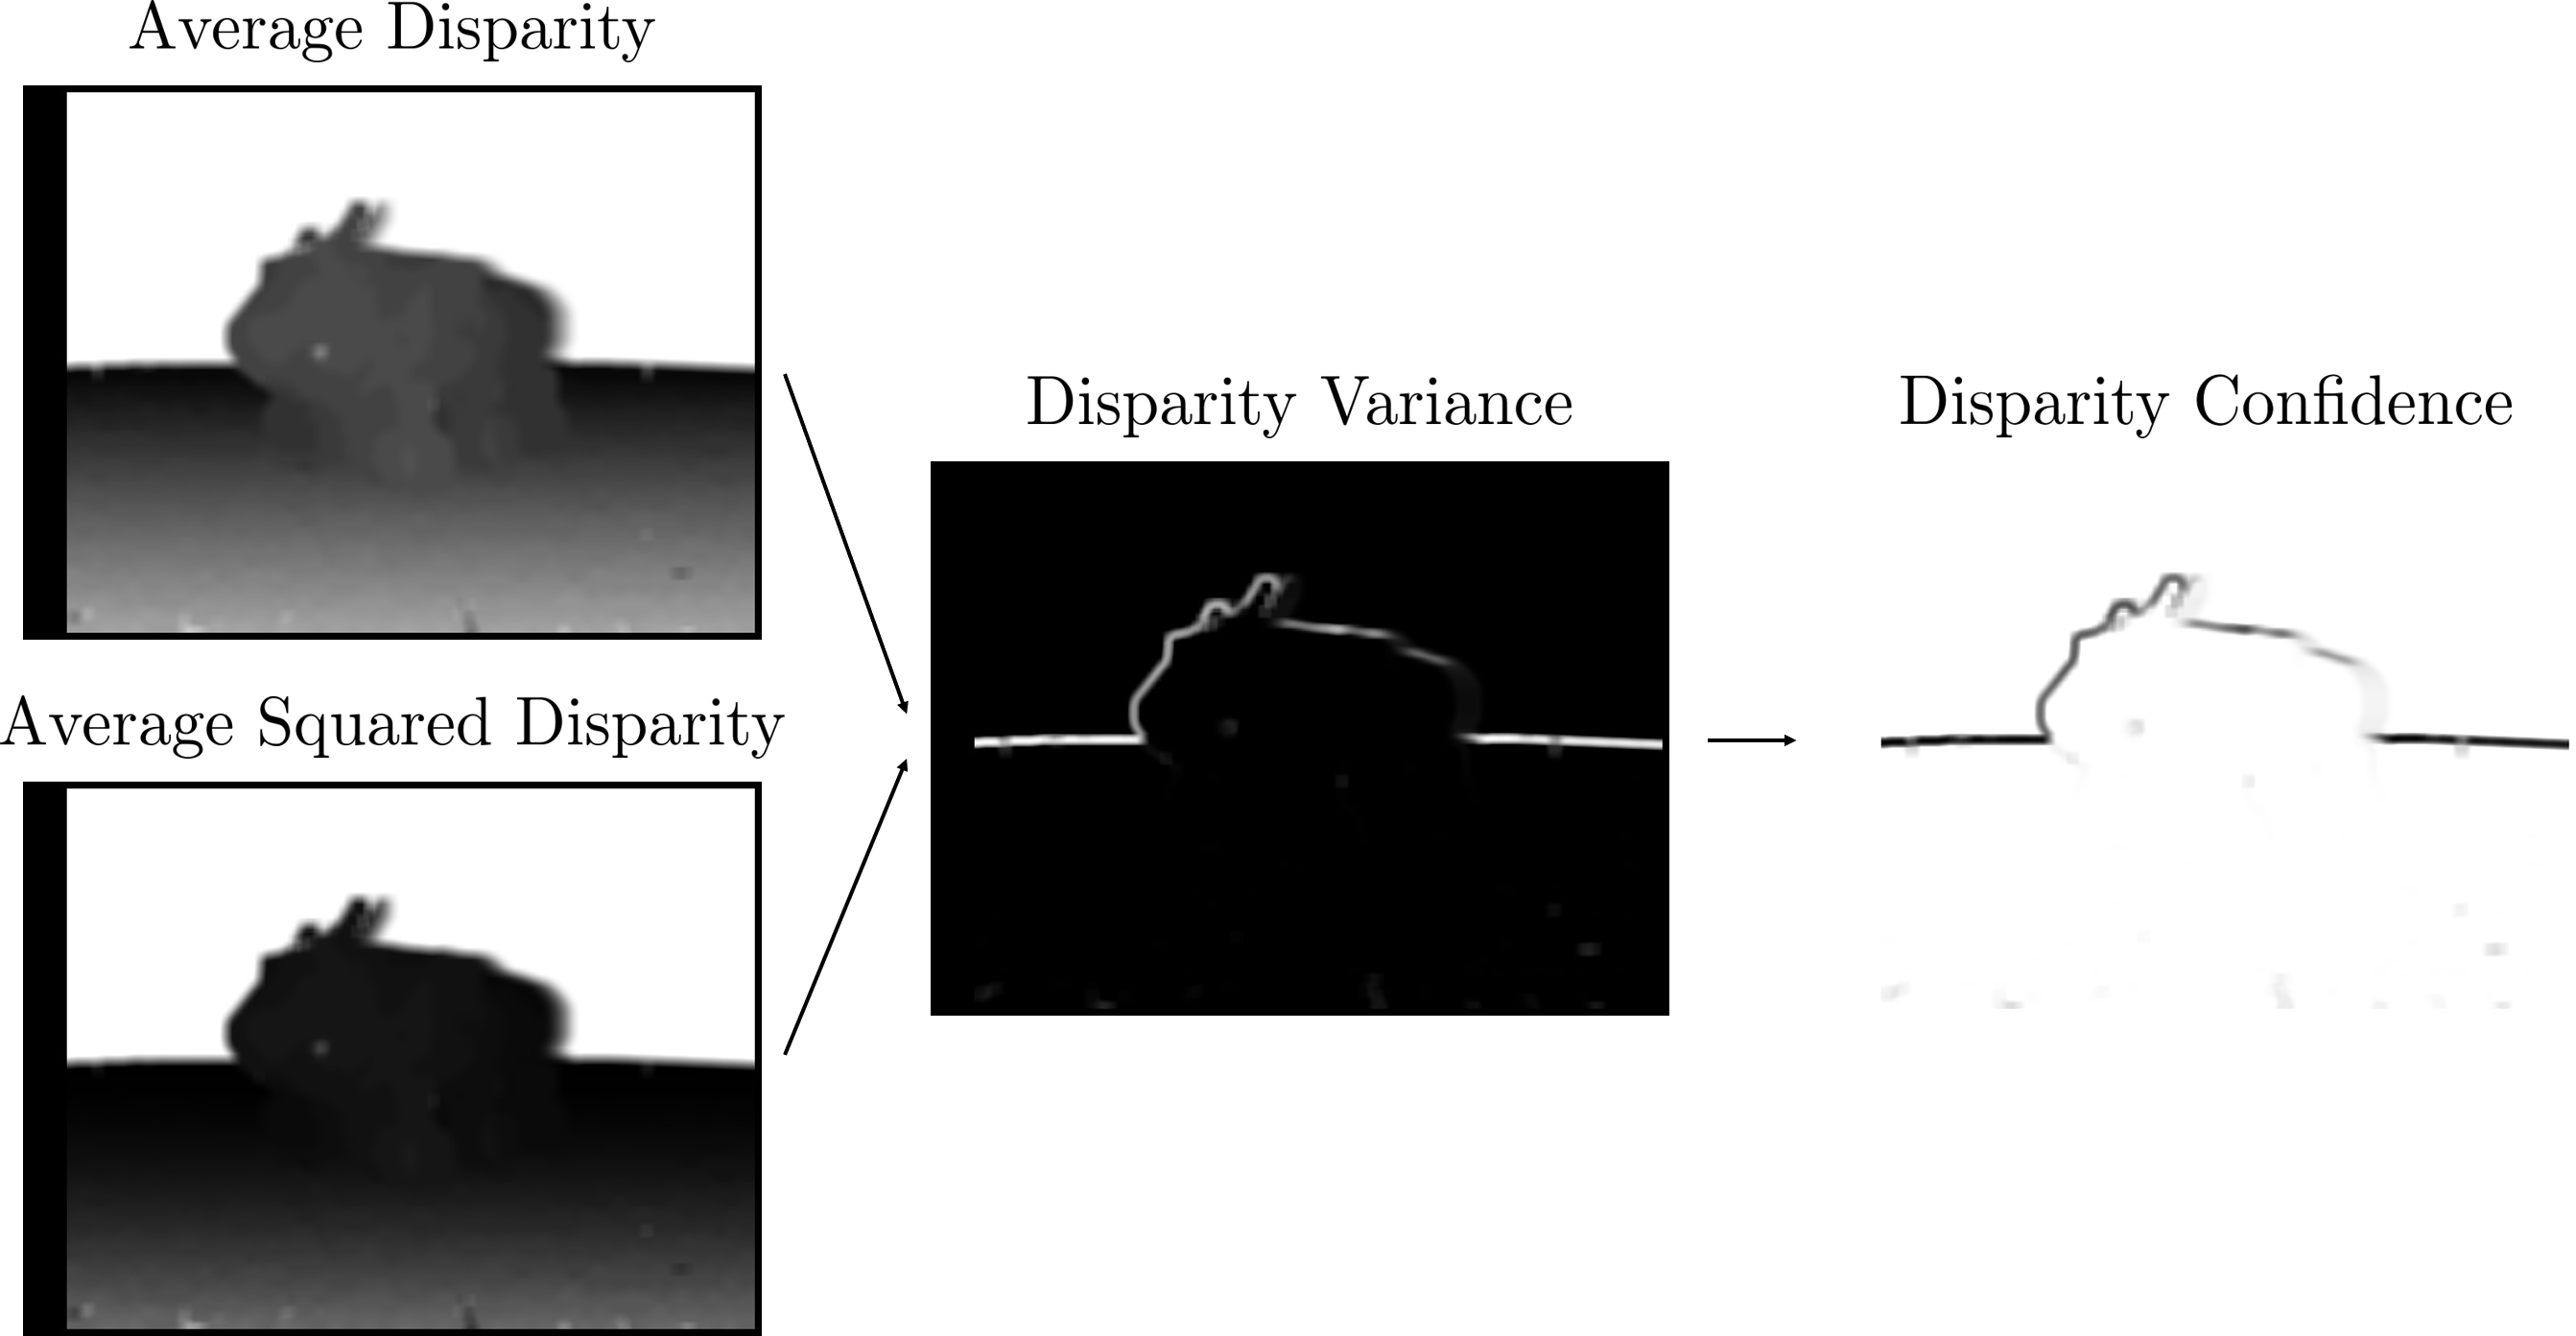
\includegraphics[scale=.28]{chapters/03_fundamentals_of_image_processing/img/confidence_map.png}
	\caption{Generation of the confidence map from the variance within the disparity map.}
	\label{fig::331_confidence_map}
\end{figure}
Before that, we further introduce an additional measure for the prevention of accidentally assigned correspondences in the initial block matching algorithm by using a left-right consistency check \cite{egnal2004stereo}. Therefore, the block matching algorithm is used in the right image, and we search for correspondences in the left image. In contrast to the computation of the left disparity map $\bm{D}_\text{left}$, for the right disparity map $\bm{D}_\text{right}$, we only need to check for correspondences along the epipolar line in the positive displacement direction. The left-right consistency $\bm{L}$ is then obtained by 
\begin{align}
	\bm{L}(x, y) = 
	\begin{cases}
	\min \left[\text{Con}(\bm{D}_\text{left})(x, y), \text{Con}(\bm{D}_\text{right})(x + d_\text{left}, y)\right] & \text{for } \Delta d < t  \\
	0 & \text{else}
	\end{cases},
\end{align}
where $d_\text{left}$ is the disparity of $\bm{D}_\text{left}$ at position $(x,y)$, and therefore represents the index shift which results from the block matching algorithm. Furthermore, if $\Delta d = \bm{D}_\text{left}(x, y) + \bm{D}_\text{right}(x + d_\text{left}, y)$ is smaller than a threshold $t$, then the left-right consistency $\bm{L}$ is taken to be the lower bound approximation of the left and right confidences. Otherwise, the consistency is taken to be false, and hence zero (figure \ref{fig::331_weighted_least_squares_disparity}). As already pointed out, the left-right consistency, which is nothing but a confidence measure, usually reveals uncertainties in textureless regions. The weighted least squares filtering that we are about to present uses this fact to its advantage. In a first step, a consistency weighted disparity map $\bm{C}$ is computed via equation \ref{eq::331_cwd} (figure \ref{fig::331_weighted_least_squares_disparity}).
\begin{align}
	\bm{C}=\bm{L}\cdot\bm{D}_\text{left},
	\label{eq::331_cwd}
\end{align}
where $\cdot$ is an element-wise multiplication. Further, the weighted least squares filter is based on the idea of a bilateral filter \cite{tomasi1998bilateral}, and it will try to minimize an energy function $J(\bm{U})$, which takes the original grayscale image as guidance to compute a weight $w_{p,q}$ for neighboring pixels $p$, and $q$ as follows
\begin{align}
	w_{x,y,i,j}(g) = exp(-|g_{x,y}-g_{i,j}|/\sigma).
	\label{eq::331_weight}
\end{align}
Depending on the range parameter $\sigma$, this weight will be high for similar neighboring pixels of the grayscale image $g$, and therefore lead to huge costs in the following energy function $J(\bm{U})$ that we try to minimize
\begin{align}
	J(\bm{U}) = \sum_{x,y}\left[(u_{x,y}-c_{x,y})^2+\lambda\sum_{(i,j)\in\mathcal{N}(x,y)}w_{x,y,i,j}(g)(u_{x,y}-u_{i,j})^2\right],
	\label{eq::331_energy_function}
\end{align}
where $c_{x,y}$ are single pixels of the consistency weighted disparity map. The formulation of this energy function results in a solution $\bm{U}$ that encourages the propagation of disparity values from high- to low-confidence regions (figure \ref{fig::331_weighted_least_squares_disparity}). Additionally, the weight $w$, together with the smoothing parameter $\lambda$, ensure to have similar disparity values in regions with similar texture. The final disparity map $\bm{D}_\text{final}$ is then obtained by normalizing the resulting image $\bm{U}$ with
\begin{align}
	\bm{D}_\text{final} = \frac{\bm{U}}{\text{WLS}(\bm{L})},
	\label{eq::331_wls_final}
\end{align}
where $\text{WLS}(\bm{U})$ is the weighted least squares filtered version of the left-right consistency $\bm{L}$.
\begin{figure}[h!]
	\centering
	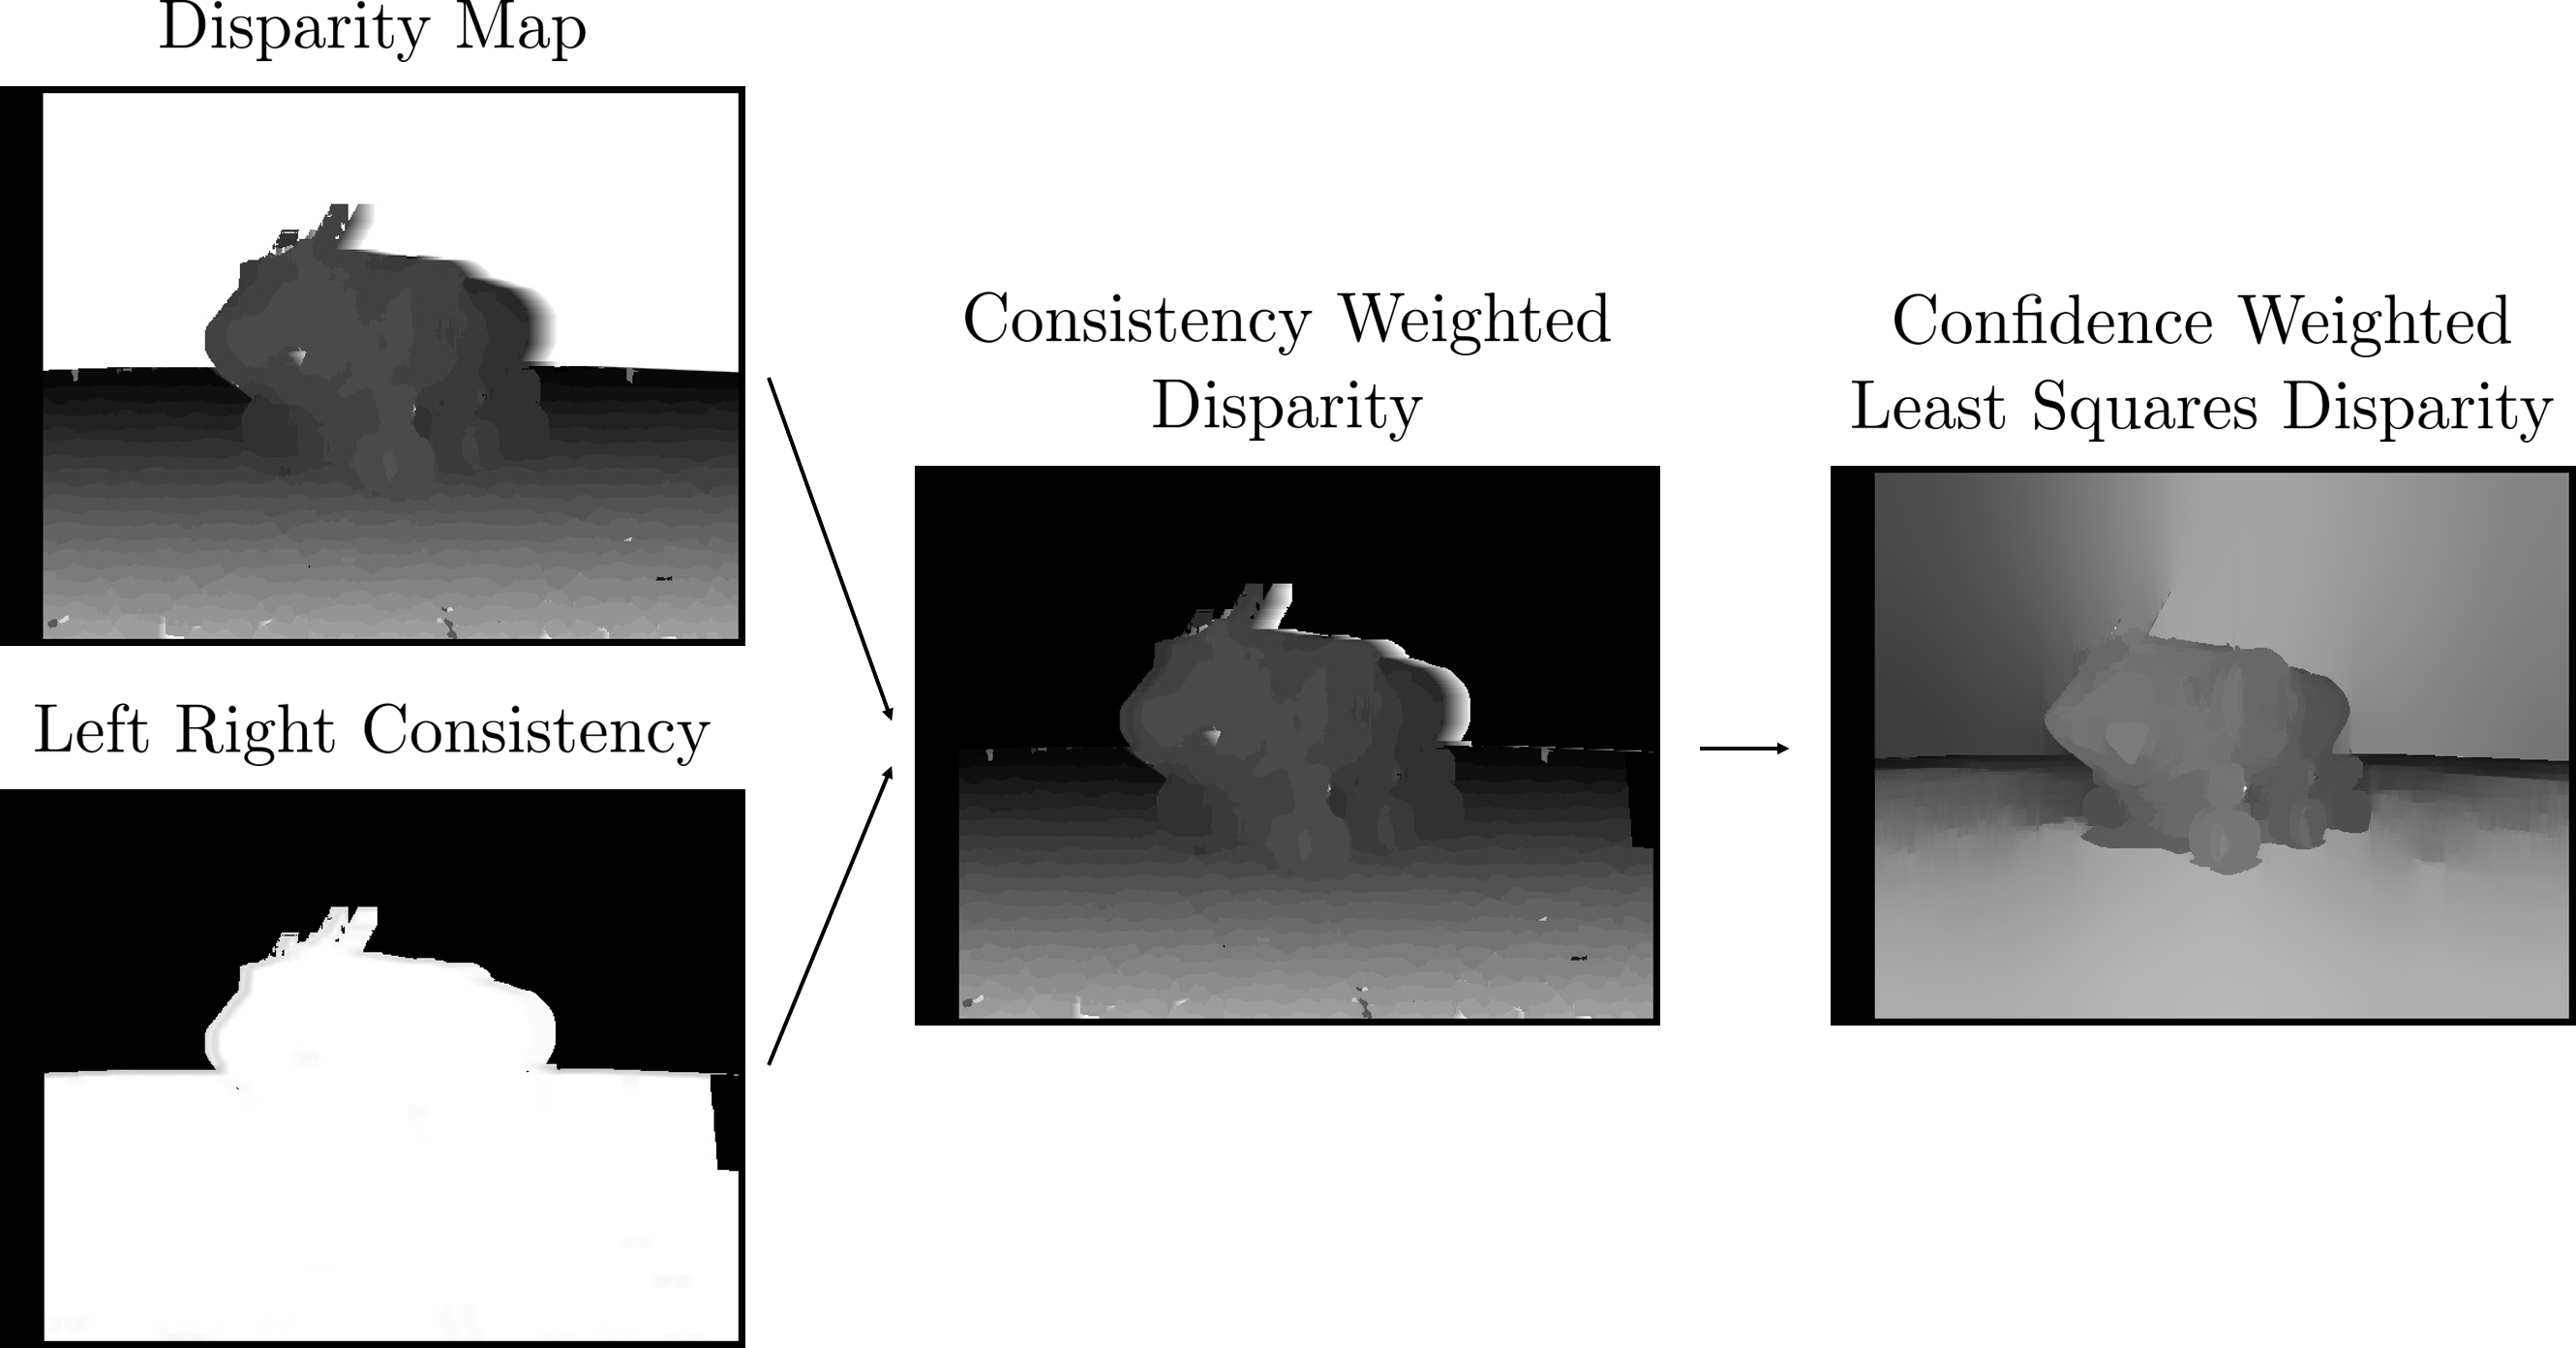
\includegraphics[scale=.28]{chapters/03_fundamentals_of_image_processing/img/weighted_least_squares_disparity.png}
	\caption{Generation of the confidence weighted least squares disparity from the disparity map, and the left-right consistency.}
	\label{fig::331_weighted_least_squares_disparity}
\end{figure}
\\\\
As already mentioned in figure \ref{fig::331_stereo_camera}, the assumption of an only translated stereo camera pair is rarely correct. Besides, there exist camera intrinsics that deform the observed image, and so the epipolar lines. Therefore, as a requirement for the algorithm to work properly, it is important to calibrate the robot's cameras. The next chapter - Mono and Stereo Camera Calibration, will explain in detail how this is done.
\FloatBarrier
\subsection{Mono and Stereo Camera Calibration}
To correct images, as we observe them with a camera, it is required to have a mathematical description of it. A simple one for a camera is the pinhole model, which is shown in figure \ref{fig::332_pin_hole_camera}. For a pinhole camera model, the image plane lies behind the coordinate frame of the camera, and is turned the other way around, but it is easier to describe the image in a virtual plane, which is located at a distance $f$ along the $z_c$-axis, where $f$ is the focal length.
\begin{figure}[h!]
	\centering
	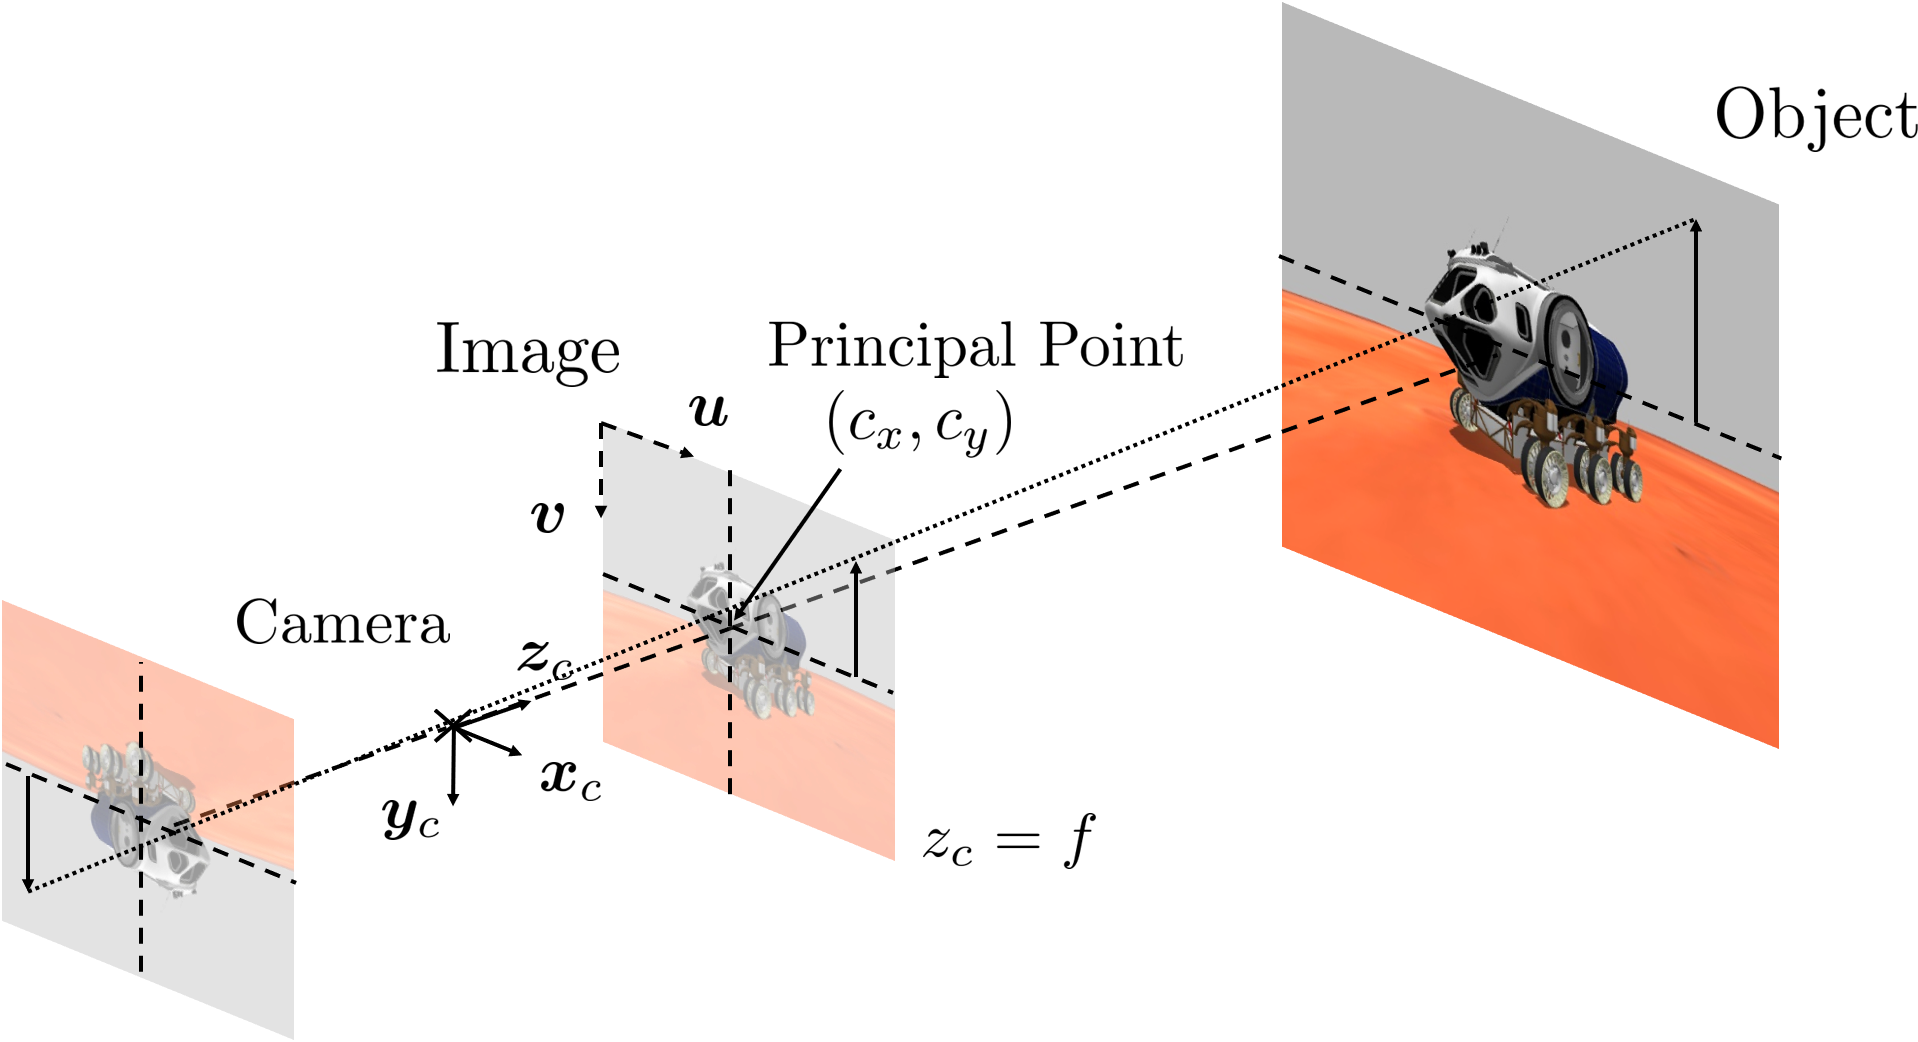
\includegraphics[scale=.28]{chapters/03_fundamentals_of_image_processing/img/pin_hole_camera.png}
	\caption{Pinhole camera model.}
	\label{fig::332_pin_hole_camera}
\end{figure}
According to the intercept theorem, a point $\bm{X}_c = (X,Y,Z)^T$ is then simply projected to the image plane by the camera matrix $\bm{K}$ with
\begin{align}
	\bm{x}_c = \bm{K}\bm{X}_c = \begin{pmatrix}
	f_x & 0   & c_x \\
	0   & f_y & c_y \\
	0   & 0   & 1
	\end{pmatrix}\bm{X}_c.
	\label{eq::332_focal_intrinsics}
\end{align}
Therein, $\bm{K}$ contains the intrinsic camera parameters, such as the focal lengths and the principal point. For a true pinhole camera $f_x = f_y =f$, but due to errors, usually two different values are chosen. The principal point lies at the position where a light ray connects perpendicularly to the image plane after passing the pinhole, and therefore just defines an offset. For a real setup, it is also required to put a lens at the pinhole's position, which adds some distortion to the image. According to \cite{duane1971close}, we model radial and tangential distortion by
\begin{align}
	x_{c,u} &= x_{c,d}(1+k_1r^2+k_2r^4+k_3r^6) + p_1(r^2+2x_{c,d}^2) + 2p_2x_{c,d}y_{c,d} 
	\label{eq::332_x_dist}\\
	y_{c,u} &= x_{c,d}(1+k_1r^2+k_2r^4+k_3r^6) + 2p_1x_{c,d}y_{c,d} + p_2(r^2+2y_{c,d}^2),
	\label{eq::332_y_dist}
\end{align}
where
\begin{align}
	(x_{c,d}, y_{c,d}) = &\,\,\text{distorted image points within the camera frame $c$,} 
	\nonumber\\
		                 &\,\,\text{as projected onto the image plane}
	\nonumber\\ 
	(x_{c,u}, y_{c,u}) = &\,\,\text{undistorted image points within the camera frame $c$,}
	\nonumber\\
	                     &\,\,\text{as projected by an ideal pinhole camera}
	\nonumber\\
	k_n = &\,\,\text{n$^\text{th}$ radial distortion coefficient}
	\nonumber\\
	p_n = &\,\,\text{n$^\text{th}$ tangential distortion coefficient}
	\nonumber\\
	r = &\,\,\sqrt{x_{c,d}^2+y_{c,d}^2}.
	\nonumber
\end{align}
Together, the focal lengths, the principal point, and the distortion coefficients make up the unknowns within our camera model. Goal of the mono camera calibration is now to find these coefficients from images of a well-known calibration pattern. Therefore, images of the calibration pattern are taken from different perspectives (figure \ref{fig::332_calibration_process}). 
\begin{figure}[h!]
	\centering
	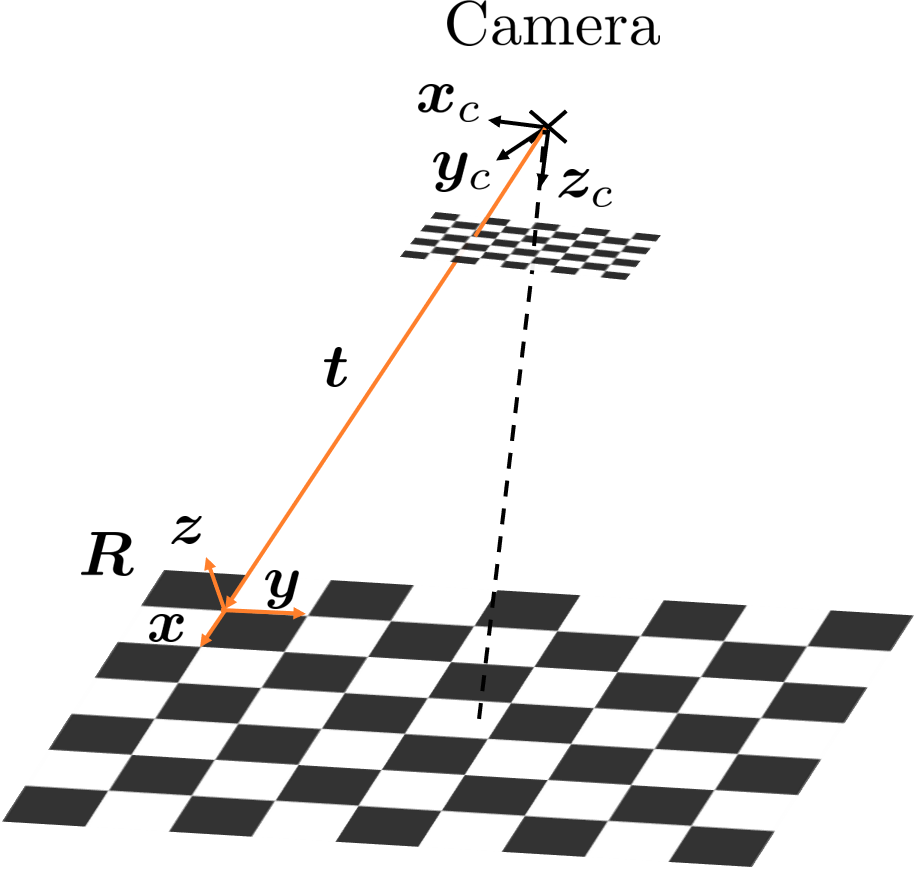
\includegraphics[scale=.28]{chapters/03_fundamentals_of_image_processing/img/calibration_process.png}
	\caption{Calibration pattern, as observed from the camera's coordinate system $C$. Within the object's coordinate system, all chessboard corners lie at a zero $z$-position.}
	\label{fig::332_calibration_process}
\end{figure}
For the mathematical description, the calibration pattern is taken to be at a fixed position and orientation, while it is assumed that the camera was moved. The position of each corner can then be described by the square's size $a$ as follows
\begin{align}
	\bm{x}_{nm} = \begin{pmatrix}
	wa & ha & 0 & 1
	\end{pmatrix}^T,
	\label{eq::332_square_size}
\end{align}
where we now switched to homogeneous coordinates, and $w\in[0,W],h\in[0,H]$ are whole numbers, corresponding to the width and the height of the pattern. It is then required to find the rotation $\bm{R}$ and translation $\bm{t}$, which transforms the object points to the image plane. They are estimated by solving a perspective-n-point problem \cite{fischler1981random}. Therefore, as shown in figure \ref{fig::332_distortion} (b), a corner detecting algorithm finds the corners $\bm{x}_{c,wh}$ within the image plane. Under the assumption of known intrinsic camera parameters, $\bm{x}_{c,wh}$ are then being undistorted according to equations \ref{eq::332_x_dist} and \ref{eq::332_y_dist}. 
\begin{figure}[h!]
	\centering
	\captionbox{}%
	[.4\linewidth]{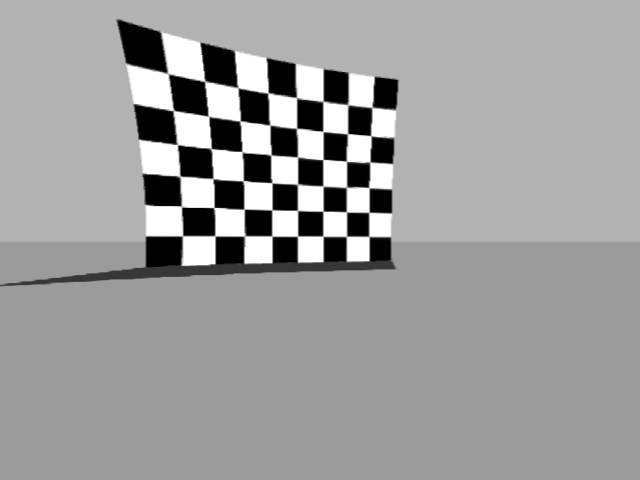
\includegraphics[scale=.2]{chapters/03_fundamentals_of_image_processing/img/gazebo_calib_left.jpg}}
	\captionbox{}%
	[.4\linewidth]{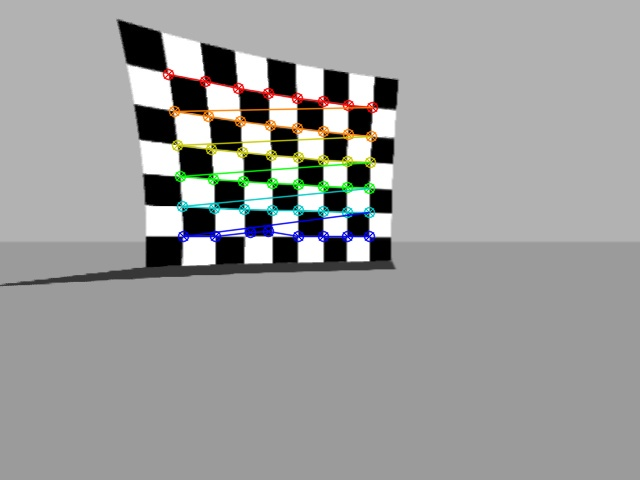
\includegraphics[scale=.2]{chapters/03_fundamentals_of_image_processing/img/gazebo_corners.jpg}}
	\caption{Distorted calibration pattern (a), and the image points as found by the algorithm (b).}
	\label{fig::332_distortion}
\end{figure} 
Each $\bm{x}_{nm}$ can then be transformed to the camera's frame, and further be projected onto the image plane via
\begin{align}
	\bm{x}_{c,wh} = \bm{K}\begin{pmatrix}
	\bm{R} & \bm{t}
	\end{pmatrix}\bm{x}_{wh},
\end{align}
where $\bm{R}$ describes the rotation, and $\bm{t}$ the translation of the camera frame to the object frame. Then, equations \ref{eq::332_x_dist} and \ref{eq::332_y_dist} are applied to obtain the undistorted image points from $\bm{x}_{c,wh}$. The undistorted image points $\bm{x}_{c,wh,u}$ are then being reprojected by inverting the rotation and translation via
\begin{align}
	\bm{x}_{wh,u} = \begin{pmatrix}
	\bm{R} & \bm{t}
	\end{pmatrix}^{-1}\bm{x}_{c,wh,u},
	\label{eq::332_reprojection}
\end{align}
from which we compute the re-projection error $\Delta x = ||\bm{x}_{wh,u} - \bm{x}_{wh}||_2$. To find the intrinsic parameters, a Levenberg-Marquardt algorithm then optimizes them in an iterative scheme to minimize the re-projection error until convergence \cite{zhang2000flexible}. The stereo camera calibration can then be performed by applying the mono camera calibration to each camera separately, from which the camera intrinsics are obtained. Given the camera intrinsics of both cameras, it is again possible to solve a perspective-n-point problem, which yields the positions and orientations of both cameras with respect to the observed object. This enables us to compute the fundamental matrix $\bm{F}$, which transforms points from the left camera's view $\bm{x}_{c_\text{left}}$, to points $\bm{x}_{c_\text{right}}$, as seen by the right camera via
\begin{align}
	\bm{x}_{c_\text{right}}^T\bm{F}\bm{x}_{c_\text{left}} = \bm{0}
\end{align}
The mapping enables us to rectify the left and the right image \cite{loop1999computing}, using the rectification transforms $\bm{R}_i$, which means that we can compute homography transforms that align epipolar lines within the images (figure \ref{fig::332_rectified}), which were previously defined by the fundamental matrix. 
\begin{figure}[h!]
	\centering
	\captionbox{}%
	[.4\linewidth]{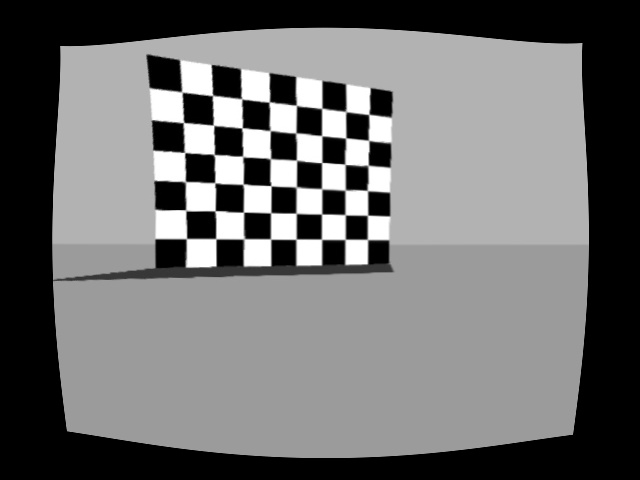
\includegraphics[scale=.2]{chapters/03_fundamentals_of_image_processing/img/gazebo_rectified_left.jpg}}
	\captionbox{}%
	[.4\linewidth]{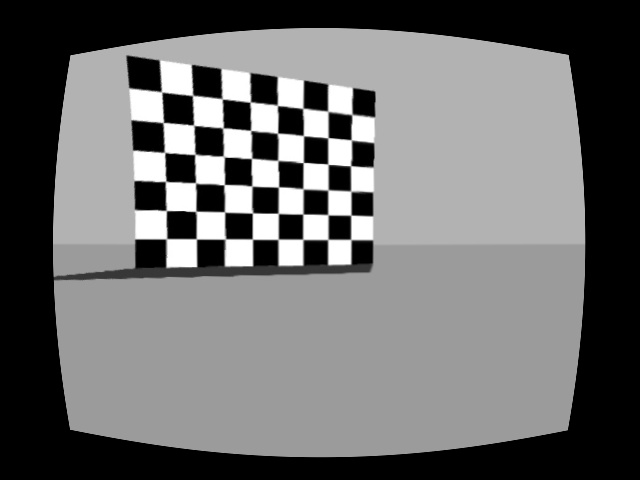
\includegraphics[scale=.2]{chapters/03_fundamentals_of_image_processing/img/gazebo_rectified_right.jpg}}
	\caption{Undistorted calibration pattern, as observed by the left camera (a), and by the right camera (b). For comparison, see the distorted calibration pattern in figure \ref{fig::332_distortion}, and note how the horizons within the images align.}
	\label{fig::332_rectified}
\end{figure}
These homography transforms map the images, as we observe them with the cameras, to a shared virtual plane, which is defined by the newly obtained projection matrices $\bm{P}_i$. Therefore, we reached our initial goal, since it enables us to apply the stereo block matching algorithm, which got introduced earlier, to the transformed images.